\documentclass[12pt]{article}

\usepackage{CJKutf8}
% 打中文時請務必加這個Package

\usepackage{epsfig,amsmath,amssymb,latexsym}
\usepackage{graphicx,epsfig,color,epsf,psfrag,hhline,amsmath,amssymb,textcomp}
\usepackage{hyperref}
\usepackage{enumitem}

\setlength {\topmargin}{-1.0in}
\setlength {\textheight}{10in}
\setlength {\oddsidemargin}{-0.25in}
\setlength {\evensidemargin}{-0.25in}
\setlength {\textwidth}{6.75in}
\setlength {\parskip}{8pt plus 2pt minus 1pt}

\newtheorem{theorem}{Theorem}[section]
\newtheorem{definition}{Definition}[section]
\newtheorem{lemma}{Lemma}[section]

\newcommand{\comb}[2]{\left (\begin{array}{c} #1 \\ #2 \end{array} \right )}

\newcommand{\inlinecomb}[2]{\mbox{\scriptsize $\left (\begin{array}{c} #1 \\ #2 \end{array} \right )$\normalsize}}

\newcommand {\bsolution}{\noindent {\em Solution:} \ }

\newcommand{\esolution}{\hfill $\Diamond$ \\ \vspace{.3cm}}

%************************** Figure**********************************
\newcommand {\bfig}[2] {\begin{figure}[htbp]
                        \centerline {
                         \epsfig{figure={#1},clip=,width={#2}}}}

\newcommand {\efig}[2]{ \caption{#2}
                        \label{fig:#1}
                        \end{figure}
                        \mymarginpar{fig:#1}}
\newcommand {\rfig}[1]{Figure \ref{fig:#1}}

%%%%%%%%%%%%%%%%%%%%%%%%%%%%%%%%%%%%%%%%%%%%%%%%%

\begin{document}
\thispagestyle{empty}
\begin{center}
{\Large \noindent COM 530500 {\bf Network Science Homework \#2} \\
\large {{\sc Due:} Thursday, November 11, 2021}  \\
}
\emph{No late homework will be accepted}.
\end{center}


\noindent {\begin{CJK}{UTF8}{bsmi}
{\bf 班級:} 資應所


\end{CJK}}

\noindent  {\begin{CJK}{UTF8}{bsmi}
{\bf 姓名:} 鄭程哲
\end{CJK}}

\noindent {\begin{CJK}{UTF8}{bsmi}
{\bf 學號:} 110065512
\end{CJK}}

\bigskip

%---------------------------------------------------------------------------
% Problem 1
%---------------------------------------------------------------------------

\noindent {\bf Problem 1.\bf(40\%)} Consider a $k$-regular undirected network (i.e., a network in which every vertex has degree $k$) with number of nodes $n$.
\begin{enumerate}[label=(\alph*)]
	\item (10\%) Show that the $n$-vector ${\bf 1}_n = [1,1,\ldots,1]$ is an eigenvector of the adjacency matrix with corresponding eigenvalue $k$. 
	\item (10\%) By making use of the fact that eigenvectors are orthogonal (or otherwise), show that there is no other eigenvector that has all elements positive. [{\it Note: The Perron-Frobenius theorem says that the eigenvector with all elements positive has the largest eigenvalue, and hence the eigenvector ${\bf 1}_n$ gives, by definition, the eigenvector centrality of our $k$-regular network and the centralities are the same for every vertex.}]
	\item (10\%) Find the {\bf Katz centralities} of all vertices in a $k$-regular network.
	\item (10\%) Find a centrality measure that can give different centralities for different vertices in a regular network. Please provide a specific example.
\end{enumerate}

\bsolution
%---------------------------------------------------------------------------
\begin{enumerate}[label=(\alph*)]
	\item The result of adjacency matrix multiplying $n$-vector $1_n$ is equal to the row sum, which means the degree of each node, i.e., $k$. Therefore, $n$-vector $1_n$ is an eigenvector of the adjacency matrix with corresponding wigenvalue $k$.
	\item Eigenvectors are orthogonal if and only if their dot product is zero. If there is other eigenvector $v$ has all elements positive, $1_n \cdot v$ must bigger than 0.
	\item Katz centralities of all vertices $x=\beta (I-\alpha A)^{-1} 1$, where $1$ is the vector $(1, 1, 1, ..., 1)^T$, $\alpha\in [0, \frac{1}{k})$, and $\beta$ is defined by the user.
	\item It's hard to answer this question. I wrote a python program (code-prob1d.ipynb) to see the centrality value of regular network with $n\in [3, 8], k\in [2, n)$. There is very tiny difference between measures. Take $n=4, k=2$ for example, PageRank gives different centralities for different vertices, i.e. 0.25, 0.24999999999999994, 0.24999999999999994, 0.25, respectively. Another example is shown in Figure 1, when $n=7, k=2$, harmonic centralities equal to 0.33333333, 0.41666667, 0.41666667, 0.41666667, 0.41666667, 0.33333333,	0.33333333, respectively. This example shows obvious difference between the centralities of vertices. However, this network isn't connected.
	\begin{figure}[h]
		\centering
		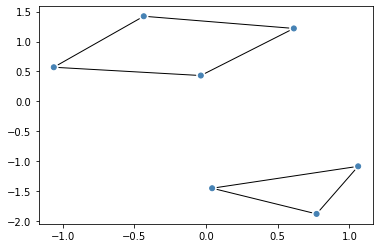
\includegraphics[width=0.5\textwidth]{fig-prob1d.png}
		\caption{2-regular network with 7 nodes.}
		\label{HW2_1}
	\end{figure}
\end{enumerate}
%---------------------------------------------------------------------------
\esolution



\newpage
%---------------------------------------------------------------------------
% Problem 2
%---------------------------------------------------------------------------
\noindent {\bf Problem 2.\bf(60\%)}
Please find a real dataset from the Internet. ({\bf Note: You need to cite the dataset in the reference.}) Note that this dataset should be an undirected network, and the total number of nodes should be greater than $500$. {\bf Please do not use the same dataset in Homework \#1.}

\begin{enumerate}[label=(\alph*)]
	\item (10\%) Briefly introduce this dataset, and list some basic statistical information, such as the number of nodes, number of edges, average clustering coefficient, diameter, average degree, maximum degree, etc.
	\item (10\%) Please visualize the dataset by plotting it. 
	\item (20\%) Please implement the Katz centrality measure (textbook chapter $7.3$ \cite{newman2010networks}) {\bf without} using the katz\_centrality function and the katz\_centrality\_numpy function provided by NetworkX, and find the top 10 nodes ranked by the Katz centrality measure you've written.
	\item (10\%) Please find the top 10 nodes by two other different centrality measures (you can use any packages and functions).
	\item (5\%) Are the top 10 nodes ranked by different centrality measures in (c) and (d) the same? Explain why?
	\item (5\%) Is there a best centrality measure for ranking this dataset? Explain why?
\end{enumerate}

\bsolution
%---------------------------------------------------------------------------
\begin{enumerate}[label=(\alph*)]
	\item The dataset I used is about real-world animal interaction network\cite{nr-aaai15}. The vertices in the network represent voles while an edge was inserted into the network whenever two voles were caught in at least one common trap over the primary trapping sessions being considered. Basic statistical information is shown below:
	\begin{itemize}
		\item Number of nodes: 1481
		\item Number of edges: 4569
		\item Average clustering coefficient: 0.522543
		\item Diameter: 18
		\item Average degree: 6.17
		\item Maximum degree: 39
	\end{itemize}
	\item Visualization is shown in Figure 2.
	\begin{figure}[h]
		\centering
		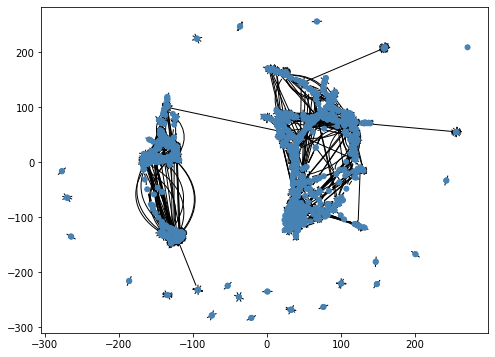
\includegraphics[width=0.5\textwidth]{fig-prob2b.png}
		\caption{Dataset visualization.}
		\label{HW2_2}
	\end{figure}
	\item I used the formula taught in class, i.e. $x(t)=\alpha Ax(t-1)+\beta$. Iterate it and get the converged Katz centrality.\\[1em]
	Top-10 nodes: [13, 62, 358, 93, 1023, 107, 321, 22, 221, 32]
	\item Eigenvector centrality top-10 nodes: [89, 193, 231, 111, 221, 196, 3, 13, 61, 22]\\[1em]
		  Closeness centrality top-10 nodes: [956, 664, 759, 758, 936, 1298, 498, 662, 663, 499]\\[1em]
		  Harmonic centrality top-10 nodes: [358, 196, 62, 61, 93, 13, 778, 192, 562, 355]\\[1em]
		  Betweenness centrality top-10 nodes: [778, 932, 928, 358, 999, 1023, 196, 973, 818, 1157]
	\item The first table below shows the number of same nodes compared to Katz centrality in top-10 and top-100 respectively. These values are quite low and the most similar one is still under 50\%. Furthermore, I compare the other four different centrality measures (directly using igraph API) and the result is shown in the second table. The value in each cell represents the number of the same nodes in top-10 and top-100. As we can see from the table, different centrality measures don't have similar results. However, I printed out the centrality values of each method and noticed that these centrality values are quite close. I think one of reason is that the central nodes are too close to each other and there is no significant difference between them. As the figure shown above, most of the nodes are crowded in the center.\\[1em]
		\begin{tabular}{|c|c|c|}
			\hline
			& Top-10 & Top-100 \\ \hline
			Eigenvector & 3      & 34      \\ \hline
			Closeness   & 0      & 15      \\ \hline
			Harmonic    & 4      & 48      \\ \hline
			Betweenness & 2      & 49      \\ \hline
		\end{tabular} \\[1em]
		\begin{tabular}{|c|c|c|c|c|}
			\hline
			            & Eigenvector & Closeness & Harmonic & Betweenness \\ \hline
			Eigenvector &             & 0 / 8     & 3 / 44   & 1 / 19      \\ \hline
			Closeness   &             &           & 0 / 40   & 0 / 30      \\ \hline
			Harmonic    &             &           &          & 3 / 53      \\ \hline
			Betweenness &             &           &          &             \\ \hline
		\end{tabular}
	\item As I described in (e), most of the centrality values are too close to distinguish even using different measures. Therefore, I think there is no best centrality measure for ranking this dataset.
\end{enumerate}
%---------------------------------------------------------------------------
\esolution

%---------------------------------------------------------------------------
% The end of problems.
%---------------------------------------------------------------------------

%---------------------------------------------------------------------------
% References
%---------------------------------------------------------------------------
\begin{thebibliography}{9}
	\bibitem{newman2010networks} 
		Newman, Mark. 
		\emph{Networks: An Introduction.} 
		Oxford University Press, 2010.
	\bibitem{nr-aaai15} 
		Ryan A. Rossi and Nesreen K. Ahmed. 
		\emph{The Network Data Repository with Interactive Graph Analytics and Visualization.}
		\url{http://networkrepository.com/}
		2015
\end{thebibliography}

\end{document}
